% jak to bude vypadat
Pro potřeby zobrazení jsem se rozhodl vytvořit velmi jednoduchou \gls{spa}. Jediné co se na ní bude nacházet budou tři 
tlačítka pro přepínání mezi jednotlivými senzory a místo pro graf hodnot. Celá aplikace bude napsaná v javascriptu. 
Nejsem v něm úplně zběhlý, takže je možné, že některé konstrukce budou neoptimální, nebo přinejmenším podivné, avšak 
nemělo by to mít vliv na funkčnost. Koncept celé aplikace vypadá takto.

\begin{figure}[H]
  \centering
  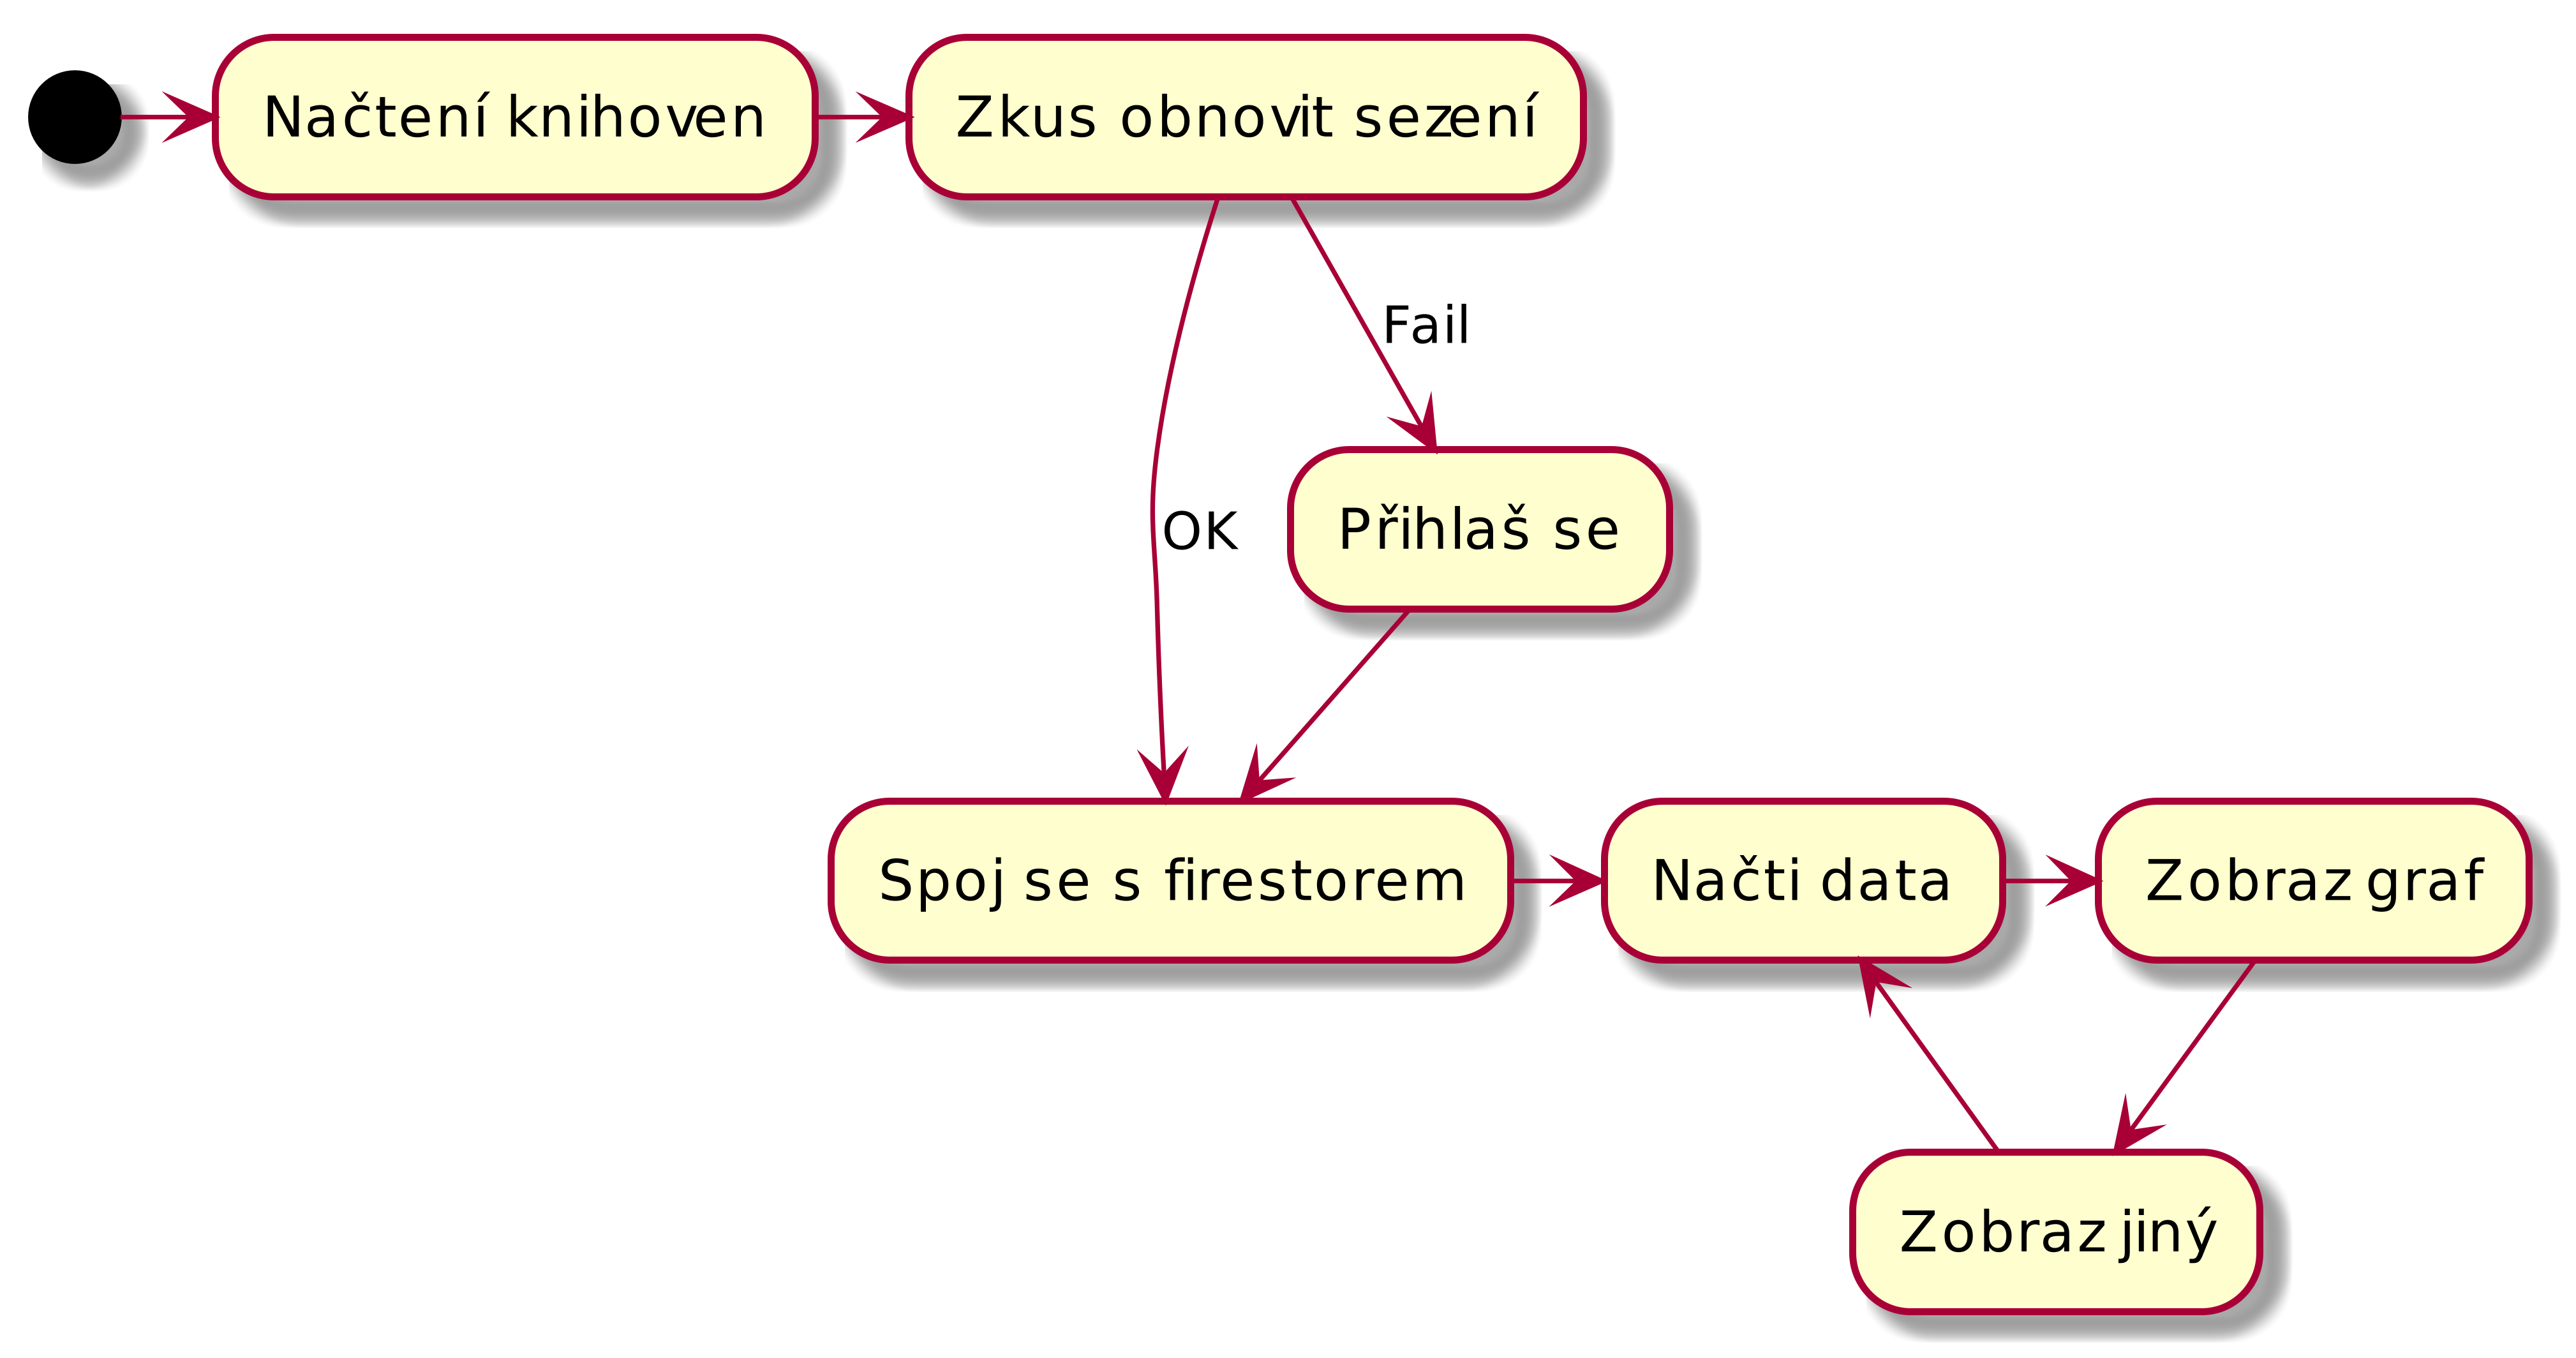
\includegraphics[width=\textwidth]{grafy.png}
  \caption{Průběh programu}
\end{figure}
